\section{2D Haar Transform}
\subsection{Implimentation}
The level 1 Haar Transform was implemented in the following way

\lstinputlisting[language=Octave]{../calcHaarLevel1.m}

\subsection{Quantizing the Haar Transform}
Using the function implemented above, I calculated the level 1 Haar Transform of the Kodim19 image. The output of the transform was then quantized using the same procedure as before with a $Q_{step}$ of 15. The inverse transforms were then calculated and are shown below in Figure \ref{fig:QuantHaarKodim}

\begin{figure}[!h]
    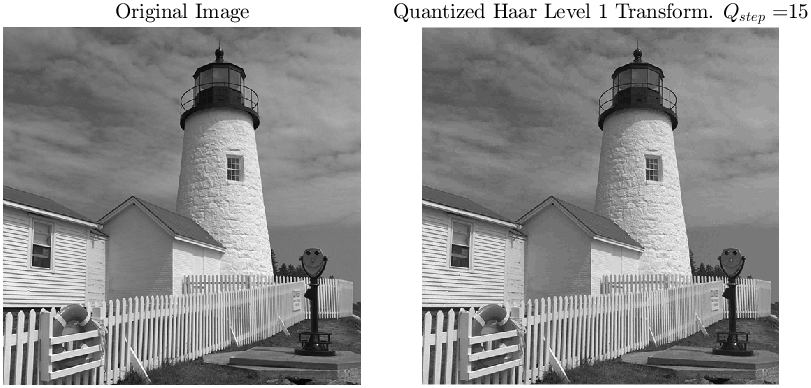
\includegraphics[width=1\textwidth]{QuantHaarKodim.png}
    \centering
    \caption{Haar and Quantized Haar Transform of Kodim19}
    \label{fig:QuantHaarKodim}
\end{figure}
\noindent The entropy calculated for the quantized haar transform of kodim19 was 1.96687 bits/pixel.

\subsection{Comparing $H_{qharr}$ and $H_{qi}$}
$H_{qharr}$ denotes the entropy of the quantized level 1 haar transform while $H_{qi}$ denotes the entropy of the quantized image. We can clearly see that the entropy of the quantized Haar transform is a lot lower than just performing normal quantization, 1.96687 as opposed to 5.845 bits/pixel. This is because of the energy compaction property of the Haar transform. By applying the transform we essentially concentrate the probability distribution around a limited number of symbols. This has the effect of lowering the overall entropy. Quantizing the symbols then further concentrates the energy leading to the lower entropy.

\subsection{Visually Comparing The Quantized Haar Transform and The Original Images}
Visually, the quantization artifacts are a lot harder to see in the quantized Haar image in Figure \ref{fig:QuantHaarKodim} when compared with the quantized image in Figure \ref{fig:QuantKodim}. Looking closely, we can still see some quantization artifacts in the form of small patches of homogeneous colors. But the effect is a lot more subtle here than in Figure \ref{fig:QuantKodim}.  